\PassOptionsToPackage{table}{xcolor}
%\documentclass{beamer}
\documentclass[compress]{beamer}
%\usetheme{Epam}
\usetheme{Copenhagen}
\usepackage{xcolor}
\usepackage{listings}
\usepackage{graphicx}
\usepackage[utf8]{inputenc}
\usepackage{datetime}
\usepackage{beamerthemesplit}
%\beamertemplatenavigationsymbolsempty
\usepackage{listingsutf8}
\usepackage{ragged2e}
\usepackage{hyperref}
\lstset{ %
  language=C,                      % the language of the code
%  basicstyle=\ttfamily,           % the size of the fonts that are used for the code
%  basicstyle=\ttfamily\tiny,      % the size of the fonts that are used for the code
  basicstyle=\ttfamily\scriptsize, % the size of the fonts that are used for the code
  numbers=left,                    % where to put the line-numbers
  numberstyle=\tiny\color{gray},   % the style that is used for the line-numbers
  stepnumber=1,                    % the step between two line-numbers. If it's 1, each line 
                                   % will be numbered
  numbersep=5pt,                   % how far the line-numbers are from the code
  %backgroundcolor=\color{gray},   % choose the background color. You must add \usepackage{color}
  showspaces=false,               % show spaces adding particular underscores
  showstringspaces=false,         % underline spaces within strings
  showtabs=false,                 % show tabs within strings adding particular underscores
%  frame=shadowbox,                   % adds a frame around the code
  rulecolor=\color{black},        % if not set, the frame-color may be changed on line-breaks within not-black text (e.g. commens (green here))
  tabsize=4,                      % sets default tabsize to 4 spaces
  captionpos=,                   % sets the caption-position to bottom
  breaklines=false,                % sets automatic line breaking
  breakatwhitespace=false,        % sets if automatic breaks should only happen at whitespace
  title=\lstname,                 % show the filename of files included with \lstinputlisting;
                                  % also try caption instead of title
  keywordstyle=\color{blue},      % keyword style
  commentstyle=\color{mygreen},   % comment style
  stringstyle=\color{magenta},    % string literal style
%  escapeinside={\%*}{*)},        % if you want to add a comment within your code
  inputencoding=utf8,
  extendedchars=\true,
  morekeywords={*,..., restrict, alignof, alignas, bool, true, false, size_t, ssize_t, inline, \_Noreturn, noreturn},
  breakautoindent=false,
  breakindent=1pt,
}

%\setbeameroption{show only notes}
%\usepackage{pgfpages}
%\setbeameroption{show notes}
%\setbeameroption{show notes on second screen=right}

\setbeamertemplate{navigation symbols}{}

\definecolor{oddrow}{RGB}{100,149,237}
\definecolor{evenrow}{RGB}{135,206,250}
\def\mybs{\textbackslash}
\newcommand{\qq}{\symbol{34}} % the decimal ascii code for "
\newcommand{\sq}{\symbol{39}} % the decimal ascii code for '

\makeatletter
\newcommand{\rmnum}[1]{\romannumeral #1}
\newcommand{\Rmnum}[1]{\expandafter\@slowromancap\romannumeral #1@}
\newcommand{\inc}{\symbol{45}\symbol{45}}
\newcommand{\dec}{\symbol{43}\symbol{43}}
\newcommand{\lsh}{\symbol{60}\symbol{60}}
\newcommand{\rsh}{\symbol{62}\symbol{62}}
\makeatother

\newcommand{\specialcell}[2][c]{%
  \begin{tabular}[#1]{@{}c@{}}#2\end{tabular}}
\newcommand{\specialcellhl}[2][l]{%
  \begin{tabular}[#1]{@{}l@{}}#2\end{tabular}}
\newcommand{\specialcellhc}[2][c]{%
  \begin{tabular}[#1]{@{}c@{}}#2\end{tabular}}

\definecolor{mygreen}{rgb}{0,0.6,0}
\definecolor{olive}{rgb}{0.3, 0.4, .1}
\definecolor{fore}{RGB}{249,242,215}
\definecolor{back}{RGB}{51,51,51}
\definecolor{title}{RGB}{255,0,90}
\definecolor{dgreen}{rgb}{0.,0.6,0.}
\definecolor{gold}{rgb}{1.,0.84,0.}
\definecolor{JungleGreen}{cmyk}{0.99,0,0.52,0}
\definecolor{BlueGreen}{cmyk}{0.85,0,0.33,0}
\definecolor{RawSienna}{cmyk}{0,0.72,1,0.45}
\definecolor{Magenta}{cmyk}{0,1,0,0}

\newcommand{\kwblue}[1]{\texttt{\textcolor{blue}{#1}}}
\newcommand{\kwblack}[1]{\texttt{\textcolor{black}{#1}}}
\newcommand{\kwred}[1]{\texttt{\textcolor{red}{#1}}}
\newcommand{\kwmagenta}[1]{\texttt{\textcolor{Magenta}{#1}}}

%\newcommand{\hdr}[1]{\textless{#1}\textgreater{}}
\newcommand{\hdr}[1]{\textless{\kwmagenta{#1}}\textgreater{}}

\author[\href{mailto:vasili_slapik@epam.com}{Vasili Slapik}]{\texorpdfstring{Vasili Slapik\newline\href{mailto:vasili_slapik@epam.com}{vasili\_slapik@epam.com}}{Vasili Slapik}}


\title{\Rmnum{2}. Program structure and variables}

\begin{document}

%TODO: const vars has external linkage in C but internal in C++ (as with static)
%TODO: tentative definitions for variables
%TODO: float points representation and limits (precision loss)
%TODO: endianness? here?

%%%%%%%%%%%%%%%%%%%%%%%%%%%%%%%%%%%%%%%%%%%%%%%%%%%%%%%%%%%%%%%%%%%%%%%%%%%%%%%%%
\frame{\titlepage}
%%%%%%%%%%%%%%%%%%%%%%%%%%%%%%%%%%%%%%%%%%%%%%%%%%%%%%%%%%%%%%%%%%%%%%%%%%%%%%%%%%
\begin{frame}{Variables}
    \only<1>{
        \begin{itemize}
            \item identifiers are case sensitive
            \item identifiers must start with a letter
            \item should not start with an underscore
            \item should consist of 31 or fewer characters to ensure portability
            \item should not be a keyword
        \end{itemize}
    }
\end{frame}
%%%%%%%%%%%%%%%%%%%%%%%%%%%%%%%%%%%%%%%%%%%%%%%%%%%%%%%%%%%%%%%%%%%%%%%%%%%%%%%%%
\begin{frame}{C language keywords}
    \begin{center}
        \rowcolors{1}{oddrow}{evenrow}
        \begin{tabular}{l|l|l}
            \texttt{auto}        &     \texttt{if}                &     \texttt{unsigned}                \\
            \texttt{break}       &     \texttt{inline (C99)}      &     \texttt{void}                    \\
            \texttt{case}        &     \texttt{int}               &     \texttt{volatile}                \\
            \texttt{char}        &     \texttt{long}              &     \texttt{while}                   \\
            \texttt{const}       &     \texttt{register}          &     \texttt{\_Alignas (C11)}         \\
            \texttt{continue}    &     \texttt{restrict (C99)}    &     \texttt{\_Alignof (C11)}         \\
            \texttt{default}     &     \texttt{return}            &     \texttt{\_Atomic (C11)}          \\
            \texttt{do}          &     \texttt{short}             &     \texttt{\_Bool (C99)}            \\
            \texttt{double}      &     \texttt{signed}            &     \texttt{\_Complex (C99)}         \\
            \texttt{else}        &     \texttt{sizeof}            &     \texttt{\_Generic (C11)}         \\
            \texttt{enum}        &     \texttt{static}            &     \texttt{\_Imaginary (C99)}       \\
            \texttt{extern}      &     \texttt{struct}            &     \texttt{\_Noreturn (C11)}        \\
            \texttt{float}       &     \texttt{switch}            &     \texttt{\_Static\_assert (C11)}  \\
            \texttt{for}         &     \texttt{typedef}           &     \texttt{\_Thread\_local (C11)}   \\
            \texttt{goto}        &     \texttt{union}             &
        \end{tabular}
    \end{center}
\end{frame}
%%%%%%%%%%%%%%%%%%%%%%%%%%%%%%%%%%%%%%%%%%%%%%%%%%%%%%%%%%%%%%%%%%%%%%%%%%%%%%%%%
\begin{frame}{Constants and literals}
    The constants refer to fixed values that the program may not alter during its execution. These fixed values are also called literals.
    \begin{itemize}
        \item numeric
            \begin{itemize}
                \item decimal: \textbf{1234}
                \item octal: \textbf{01234}, \textbf{0}
                \item hexadecimal: \textbf{0x1234}
                \item floating-point: \textbf{123.456e-67}
                \item hexadecimal floating-point: \textbf{0xf.4p2} (0xf.4$\times{2}^2$ = 61) (C99)
            \end{itemize}
        \note{character constants have type int}
        \item character: \textbf{'A'}
        \item string: \textbf{"A"}, \textbf{"Hello world"}
    \end{itemize}
\end{frame}
%%%%%%%%%%%%%%%%%%%%%%%%%%%%%%%%%%%%%%%%%%%%%%%%%%%%%%%%%%%%%%%%%%%%%%%%%%%%%%%%%
\begin{frame}{Constants types}
    \rowcolors{1}{oddrow}{evenrow}
    \only<1>{
        \begin{center}
            \begin{itemize}
                \item integer constants
                \begin{tabular}{lll}
                    no suffix    & \texttt{44}    & \textbf{int}           \\
                    \texttt{U}   & \texttt{55U}   & \textbf{unsigned int}  \\
                    \texttt{L}   & \texttt{66L}   & \textbf{long int}      \\
                    \texttt{LL}  & \texttt{77LL}  & \textbf{long long int} \\
                \end{tabular}
            \end{itemize}
            \begin{itemize}
                \item float-point constants
                \begin{tabular}{lll}
                    no suffix    & \texttt{4.0}   & \textbf{double}        \\
                    \texttt{F}   & \texttt{6.6F}  & \textbf{float}         \\
                    \texttt{L}   & \texttt{75e3L} & \textbf{long double}   \\
                \end{tabular}
            \end{itemize}
            \begin{itemize}
               \item All letters in integer literals are case-insensitive, \texttt{0xDeAdBaBeU} and \texttt{0XdeadBABEu} represent the same number.
            \end{itemize}
        \end{center}
    }
    \only<2>{
        \lstinputlisting{02_constant_types.c}
    }
\end{frame}
%%%%%%%%%%%%%%%%%%%%%%%%%%%%%%%%%%%%%%%%%%%%%%%%%%%%%%%%%%%%%%%%%%%%%%%%%%%%%%%%%
\begin{frame}{Defining constants}
    \begin{itemize}
        \item using \textbf{\#define} macro
        \lstinputlisting{02_const_macro.c}
        \item using \textbf{const} keyword
        \lstinputlisting{02_const_const.c}
        \item using \textbf{enum} keyword
        \lstinputlisting{02_const_enum.c}
        %enums are signed (compatible with int). In any context where an unsigned type is required (think especially bitwise operations!), enums are out.
        %if long long is wider than int, big constants won't fit in an enum.
        %The size of an enum is sizeof(int). For arrays of small values (up to say, CHAR_MAX) you might want a char foo[] rather than an enum foo[] array.
        %enums are integral numbers. You can't have enum funny_number { 3.14, 2.71 }.
        %enums are a C89 feature; K&R compilers (admittedly ancient) don't understand them.
    \end{itemize}
\end{frame}
%%%%%%%%%%%%%%%%%%%%%%%%%%%%%%%%%%%%%%%%%%%%%%%%%%%%%%%%%%%%%%%%%%%%%%%%%%%%%%%%%
\begin{frame}{How constant is const?}
    \begin{itemize}
        \only<1>{
            \item First experiment
            \lstinputlisting{02_changing_const_1.c}
        }
        \only<2>{
            \item Second experiment
            \lstinputlisting{02_changing_const_2.c}
        }
        \only<3>{
            \item A little change
            \lstinputlisting{02_changing_const_3.c}
        }
    \end{itemize}
\end{frame}
%%%%%%%%%%%%%%%%%%%%%%%%%%%%%%%%%%%%%%%%%%%%%%%%%%%%%%%%%%%%%%%%%%%%%%%%%%%%%%%%%
\begin{frame}{Backslash escapes}
    \begin{tabular}{ll}
        \mybs\mybs & Literal backslash \\
        \mybs{\qq} & Double quote \\
        \mybs{\sq} & Single quote \\
        \mybs{n} & Newline (line feed) \\
        \mybs{r} & Carriage return \\
        \mybs{b} & Backspace \\
        \mybs{t} & Horizontal tab \\
        \mybs{f} & Form feed \\
        \mybs{a} & Alert (bell) \\
        \mybs{v} & Vertical tab \\
        \mybs{?}   & Question mark (used to escape trigraphs) \\
        \mybs{nnn} & Character with octal value nnn \\
        \mybs{xhh} & Character with hexadecimal value hh \\
    \end{tabular}
\end{frame}
%%%%%%%%%%%%%%%%%%%%%%%%%%%%%%%%%%%%%%%%%%%%%%%%%%%%%%%%%%%%%%%%%%%%%%%%%%%%%%%%%
\begin{frame}{C data types}
    \note{signedness of char}
    \note{The char type is distinct from both signed char and unsigned char, but is guaranteed to have the same representation as one of them.}
    \note{mention limits.h}
    \begin{itemize}
        \item \textbf{char}: at least 8 bit, \texttt{sizeof(char) == 1}, CHAR\_BIT macro
        \item \textbf{short}: at least 16 bit, greater or equal to \texttt{sizeof(char)}
        \item \textbf{int}: at least 16 bit, greater or equal to \texttt{sizeof(short)}
        \item \textbf{long}: at least 32 bit, greater or equal to \texttt{sizeof(int)}
        \item \textbf{long long}: C99, at least 64 bit, greater or equal to \texttt{sizeof(long)}
        \item \textbf{bool}: C99, at least one bit, without \hdr{stdbool.h} - \textbf{\_Bool}
        \item \textbf{float}: single precision, at least 6 decimal digits
        \item \textbf{double}: double precision, at least 10 decimal digits
        \item \textbf{long double}: extended precision if available, otherwise the same as double
        \item \textbf{signed/unsigned} modifiers (integer types and \textbf{char})
        \item \textbf{complex} modifier (real types only), C99, without \hdr{complex.h} - \textbf{\_Complex}
    \end{itemize}
\end{frame}
%%%%%%%%%%%%%%%%%%%%%%%%%%%%%%%%%%%%%%%%%%%%%%%%%%%%%%%%%%%%%%%%%%%%%%%%%%%%%%%%%
\begin{frame}{Negative values representation in C}
ISO C states that an implementation must choose one of three different representations for integral data types:
    \begin{itemize}
        \item two's complement
        \item ones' complement
        \item sign/magnitude
    \end{itemize}
\end{frame}
%%%%%%%%%%%%%%%%%%%%%%%%%%%%%%%%%%%%%%%%%%%%%%%%%%%%%%%%%%%%%%%%%%%%%%%%%%%%%%%%%
%\begin{frame}{Floating-point types in C}
%    \only<1>{
%        \lstinputlisting{010203.c}
%    }
%    \only<2>{
%        The idea is to compose a number of two main parts:
%        \begin{itemize}
%            \item significand that contains the number’s digits; negative significands represent negative numbers.
%            \item exponent that says where the decimal (or binary) point is placed relative to the beginning of the significand;
%        \end{itemize}
%    }
%    \only<3>{
%        \begin{center}
%    Majority of hardware and programming languages use floating-point numbers in the same binary formats, which are defined in the IEEE 754 standard. The usual formats are 32 (single precision) or 64 bits (double precision):
%            \rowcolors{1}{oddrow}{evenrow}
%            \begin{tabular}{c|c|c|c}
%                Precision         & Single        & Double \\ \hline
%                Total bits        &  32           & 64     \\
%                Sign bits         &  1            & 1      \\
%                Significand bits  &  23           & 52     \\
%                Exponent bits     &  8            & 11     \\
%                Smallest number   &  2 * 2\textsuperscript(-126}            & 64     \\
%                Largest number    &  2 * 2\textsuperscript{127}  & 64     \\
%            \end{tabular}
%        \end{center}
%    }
%\end{frame}
%%%%%%%%%%%%%%%%%%%%%%%%%%%%%%%%%%%%%%%%%%%%%%%%%%%%%%%%%%%%%%%%%%%%%%%%%%%%%%%%%
\begin{frame}{Common traps}
    \only<1>{
        \lstinputlisting{02_s_u_mix_3.c}
    }
    \only<2>{
        \lstinputlisting{02_ip_trap.c}
    }
    \only<3>{
        \lstinputlisting{02_s_u_mix_2.c}
    }
    \only<4>{
        \lstinputlisting{02_float_in_for_loop.c}
    }
\end{frame}
%%%%%%%%%%%%%%%%%%%%%%%%%%%%%%%%%%%%%%%%%%%%%%%%%%%%%%%%%%%%%%%%%%%%%%%%%%%%%%%%%
\begin{frame}{64 data models}
    \begin{center}
        \rowcolors{1}{oddrow}{evenrow}
        \begin{tabular}{c|c|c|c|c|l}
            Model   & int & long & \specialcell{long \\ long} & pointers & \specialcell{Sample operation \\systems} \\ \hline
            LLP64   &  32 & 32   & 64                         & 64       & \specialcellhl{MS Windows \\ (x86-64 and IA-64)} \\
            LP64    &  32 & 64   & 64                         & 64       & \specialcellhl{Most Unix and \\ Unix-like systems, \\ Solaris, Linux, \\ BSD, OS X, z/OS} \\
            ILP64   &  64 & 64   & 64                         & 64       & \specialcellhl{HAL Computer Systems \\ port of Solaris  \\ to SPARC64} \\
        \end{tabular}
    \end{center}
\end{frame}
%%%%%%%%%%%%%%%%%%%%%%%%%%%%%%%%%%%%%%%%%%%%%%%%%%%%%%%%%%%%%%%%%%%%%%%%%%%%%%%%%
\begin{frame}{C additional data types}
    \note{signess of char}
    \begin{itemize}
        \item \textbf{size\_t}, \textbf{ptrdiff\_t}
        \item \textbf{ssize\_t} (POSIX only)
        \item \textbf{int8\_t}, \textbf{int16\_t}, \textbf{int32\_t}, \textbf{int64\_t}
        \item \textbf{uint8\_t}, \textbf{uint16\_t}, \textbf{uint32\_t}, \textbf{uint64\_t}
        \item \textbf{\_\_int128\_t} and \textbf{\_\_uint128\_t} (GCC and Clang extention)
        \item ... and many others from the \hdr{stdint.h}
    \end{itemize}
\end{frame}
% visibility /extent
%%%%%%%%%%%%%%%%%%%%%%%%%%%%%%%%%%%%%%%%%%%%%%%%%%%%%%%%%%%%%%%%%%%%%%%%%%%%%%%%%
\begin{frame}{Storage classes}
    \only<1>{
        \begin{itemize}
            \item automatic
            \item static
            \item allocated
            \item register
            \item extern
            \item thread (since C11), variables declared with \textbf{\_Thread\_local} keyword (\textbf{thread\_local} if include \hdr{threads.h} header)
        \end{itemize}
    }
    \only<2>{
        \lstinputlisting{02_storage.c}
    }
\end{frame}
%%%%%%%%%%%%%%%%%%%%%%%%%%%%%%%%%%%%%%%%%%%%%%%%%%%%%%%%%%%%%%%%%%%%%%%%%%%%%%%%%
\begin{frame}{Memory layout}
    \only<1>{
        \begin{center}
            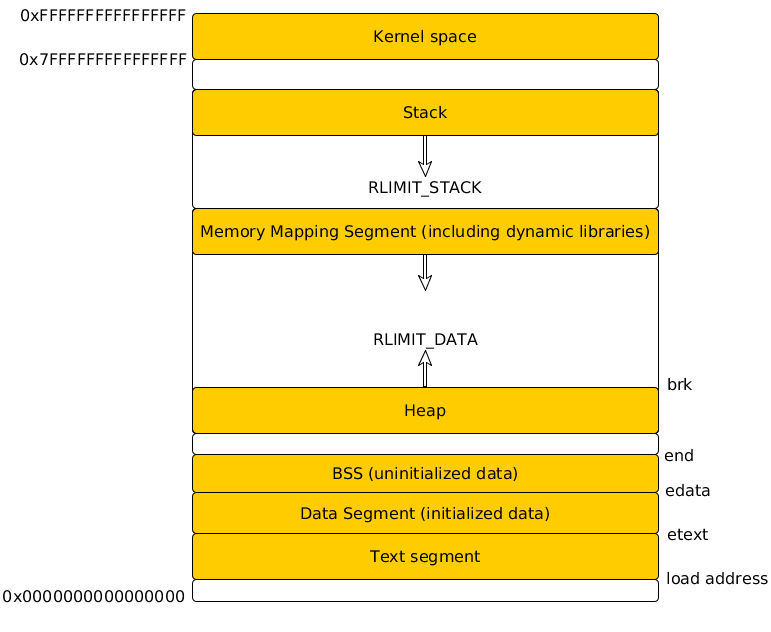
\includegraphics[height=7cm]{memlayout.png}
        \end{center}
    }
    \only<2>{
        \lstinputlisting{02_limits.c}
    }
    \only<3>{
        \lstinputlisting{02_mem_layout.c}
    }
\end{frame}
%%%%%%%%%%%%%%%%%%%%%%%%%%%%%%%%%%%%%%%%%%%%%%%%%%%%%%%%%%%%%%%%%%%%%%%%%%%%%%%%%
\begin{frame}{Summary}
    \begin{itemize}
        \item Understand data types representation.
        \item Understand run-time memory layout on your platform.
    \end{itemize}
\end{frame}
%%%%%%%%%%%%%%%%%%%%%%%%%%%%%%%%%%%%%%%%%%%%%%%%%%%%%%%%%%%%%%%%%%%%%%%%%%%%%%%

\end{document}
